\subsection{Progettazione di dettaglio e codifica}
Questo periodo inizia il giorno dopo la \textit{Revisione di Progettazione}(16/03/2019) e si conclude
con la consegna dei documenti per la \textit{Revisione di Qualifica}(12/04/2019). Le attività principali sono:
\begin{itemize}
	\item{\textbf{Incremento e Verifica:} all’inizio del periodo vengono svolte attività di Incremento e Verifica su vari documenti;}
	\item{\textbf{Glossario:} questa attività comprende sia il miglioramento del Glossario che l’aggiunta di nuovi termini;}
	\item{\textbf{Codifica:} questa attività consiste nella scrittura del codice e nella sua verifica secondo quanto indicato nella \textit{Definizione di Prodotto};}
	\item{\textbf{Lettera di presentazione:} questa attività prevede la stesura della lettera
		di presentazione per la \textit{Revisione di Qualifica}.}
\end{itemize}

\begin{figure}[h!]
	\centering
	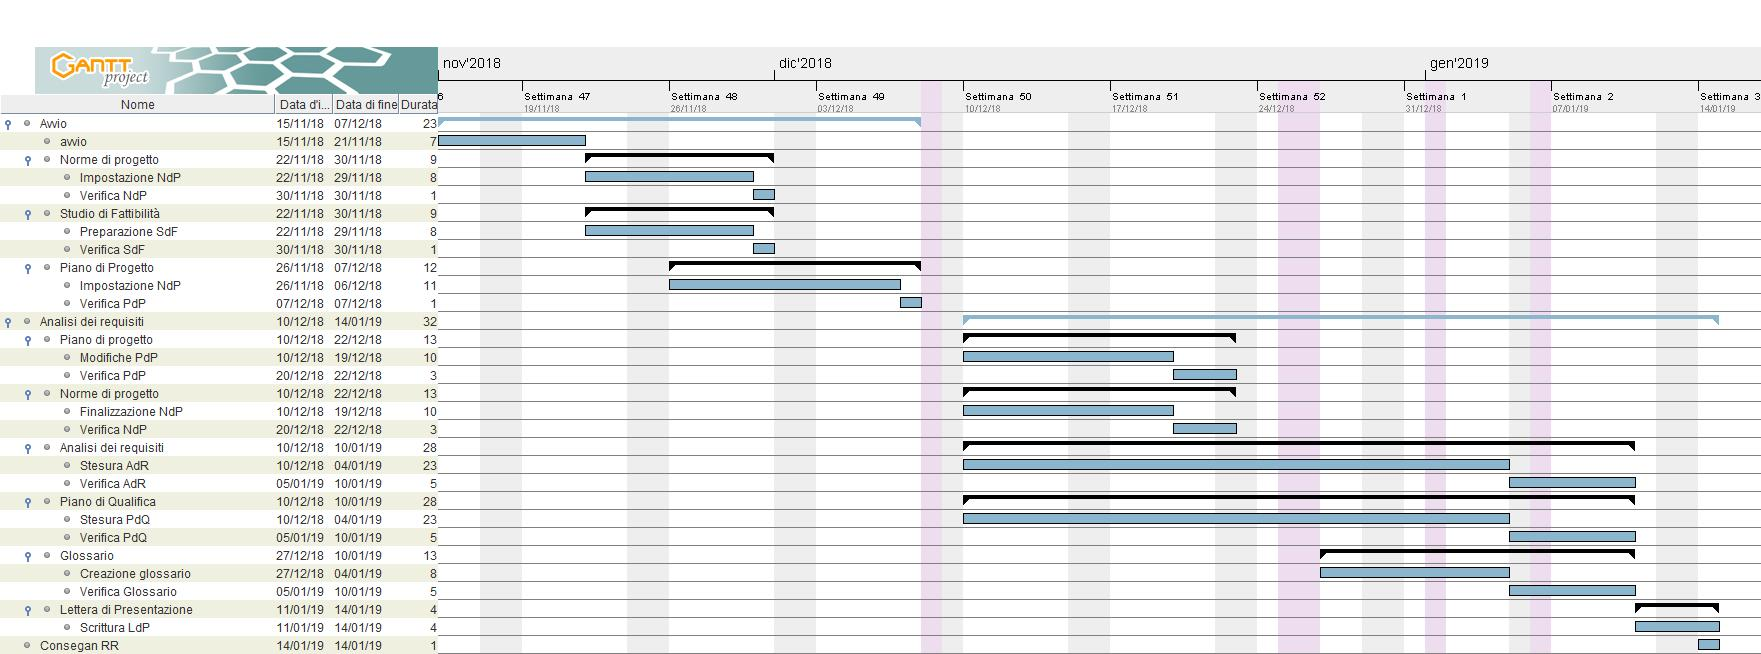
\includegraphics[width=\textwidth]{Gantt_terza_fase.jpg}
	\caption{Diagramma di Gantt per la fase fino alla Revisione di Qualifica}
\end{figure}

\begin{figure}[h!]
	\centering
	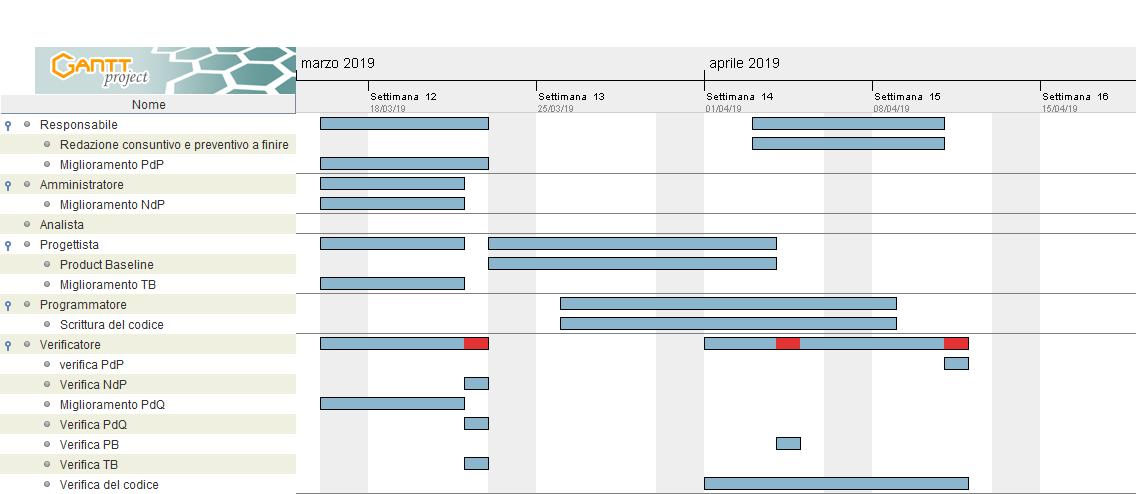
\includegraphics[width=\textwidth]{Gantt_terza_fase_risorse.jpg}
	\caption{Diagramma di Gantt delle risorse fino alla Revisione di Qualifica}
\end{figure}

\begin{tabular}{|l|l|l|}
	\hline
	\multicolumn{3}{|c|}{\textbf{Suddivisione temporale}}\\
	\hline
	\textbf{Ruolo} & \textbf{16/03/19 - 29/03/19} & \textbf{29/03/19 - 12/04/19} \\
	\hline
	\textbf{Responsabile} & \gia & \mar \\
	\hline
	\textbf{Amministratore} & \mar & \mat  \\
	\hline
	\textbf{Analista} & &  \\
	\hline
	\textbf{Progettista} & \pie \mic \daG &  \\
	\hline
	\textbf{Programmatore} & \mat \daL & \pie \daG \gia \\
	\hline
	\textbf{Verificatore} &  & \mic \daL \\
	\hline
\end{tabular}